% =============================================================================
% AgentProbe — Draft Paper for BDCC (MDPI)
% Big Data and Cognitive Computing
% =============================================================================
\documentclass[bdcc,article,submit,moreauthors,pdftex]{mdpi}

% MDPI internal commands
\firstpage{1}
\makeatletter
\setcounter{page}{\@firstpage}
\makeatother
\pubvolume{1}
\issuenum{1}
\articlenumber{0}
\pubyear{2026}
\copyrightyear{2026}
\datereceived{}
\dateaccepted{}
\datepublished{}
% ---- Additional packages (not loaded by mdpi.cls) ---------------------------
\usepackage{listings}
\usepackage{algorithm}
\usepackage{algpseudocode}

% ---- Code listing style ------------------------------------------------------
\lstset{
  basicstyle=\ttfamily\small,
  keywordstyle=\color{blue}\bfseries,
  commentstyle=\color{gray},
  stringstyle=\color{red!70!black},
  breaklines=true,
  frame=single,
  numbers=left,
  numberstyle=\tiny\color{gray},
  language=Python
}

% ---- Draft helpers -----------------------------------------------------------
\newcommand{\todo}[1]{\textcolor{red}{\textbf{[TODO: #1]}}}
\newcommand{\agentprobe}{\textsc{AgentProbe}}

% ==============================================================================
\Title{AgentProbe: Systematic Fault Injection and Observability for Evaluating the Reliability of LLM-Based Intelligent Agents}

\Author{Chhayank Jain $^{1,*}$, Sarthak Pattnaik $^{2}$ and Eugene Pinsky $^{2}$}

\AuthorNames{Chhayank Jain, Sarthak Pattnaik and Eugene Pinsky}

\address{%
  $^{1}$ \quad Arizona State University, Tempe, AZ, USA; cjain10@asu.edu\\
  $^{2}$ \quad Boston University, Boston, MA, USA; spattna1@bu.edu (S.P.); epinsky@bu.edu (E.P.)
}

\corres{Correspondence: cjain10@asu.edu}

% ==============================================================================
% Abstract — keep it simple (no custom macros) so hyperref PDF metadata works
% ==============================================================================
\abstract{
LLM-based intelligent agents are increasingly deployed in production systems, yet their reliability under adverse conditions remains poorly characterized. We present AgentProbe, an open-source fault-injection and observability toolkit for systematically evaluating agent resilience. AgentProbe implements a five-category failure taxonomy---tool call faults, orchestration errors, context degradation, latency anomalies, and output consistency violations---with configurable injectors, OpenTelemetry-based tracing, and 55 standardized benchmark tasks spanning tool use, retrieval-augmented generation, and multi-agent coordination.
%
We apply AgentProbe to compare three agent frameworks---LangGraph, LangChain, and AutoGen---across 1{,}050 experiment runs (3 frameworks $\times$ 3 task types $\times$ 5 fault conditions $\times$ 10--30 runs) using Llama~3.1 8B via Ollama. Under fault injection, LangGraph and LangChain exhibit a 12.9\% failure rate [95\% CI: 10.1--16.3\%] with 79\% recovery, while AutoGen reports 0\% failures---a statistically significant difference ($p < 0.0001$, Cohen's $h = 0.73$). Trace analysis reveals that AutoGen's apparent resilience masks complete tool-execution bypass: the LLM responds without invoking tools, constituting a silent failure mode. LangGraph and LangChain show no significant difference ($p = 1.0$), recovering more effectively from rate-limit and API errors (86\%) than from timeouts and malformed outputs (73\%). These findings demonstrate that conventional pass/fail metrics can obscure critical architectural weaknesses, and that systematic fault injection is essential for evaluating agent reliability.
}

\keyword{
  intelligent agents;
  multi-agent systems;
  agent-oriented architectures;
  Large Language Models (LLMs);
  Chain of Thought (CoT);
  reliability benchmarking;
  fault injection;
  observability;
  sub-symbolic artificial intelligence
}

% ==============================================================================
\begin{document}

% ============================================================================
\section{Introduction}\label{sec:introduction}
% ============================================================================

The concept of intelligent agents---autonomous software entities that perceive their environment and act upon it to achieve delegated goals---has been a central thread in artificial intelligence research since the foundational work of McCarthy and Minsky~\cite{wooldridge2009introduction}. The agent-oriented paradigm, consolidated in the mid-1990s after two periods of reduced AI research activity, established a rigorous framework in which agents are characterized by autonomy, reactivity, proactivity, and social ability~\cite{wooldridge1995intelligent}. The Beliefs--Desires--Intentions (BDI) architecture emerged as a dominant model for rational decision-making, grounding agent behavior in a formalism derived from practical reasoning~\cite{rao1995bdi}.

A new generation of intelligent agents has emerged with the advent of Large Language Models (LLMs). These \emph{AI agents} employ LLMs as reasoning engines, using architectures such as ReAct~\cite{yao2023react} and Chain of Thought (CoT)~\cite{wei2022chain} prompting to interleave reasoning with action execution. Unlike their symbolic BDI predecessors, these sub-symbolic agents derive their capabilities from statistical patterns learned during pre-training, enabling remarkable flexibility but introducing novel failure modes that lack formal characterization.

The deployment of LLM-based agents in production Internet-facing systems has accelerated rapidly. Agent-oriented frameworks such as LangGraph~\cite{langgraph2024}, LangChain~\cite{langchain2023}, and AutoGen~\cite{wu2023autogen} enable developers to build sophisticated multi-agent systems that coordinate tool use, retrieval-augmented generation (RAG), and inter-agent communication. However, the reliability of these systems under adverse conditions remains poorly understood. Production incident reports reveal recurring failure patterns---API timeouts cascading through agent loops, context window overflow causing hallucinated histories, orchestration deadlocks in multi-agent handoffs---yet no systematic methodology exists for reproducing, measuring, and comparing these failure modes across frameworks.

This paper addresses this gap with three contributions:

\begin{enumerate}
  \item \textbf{A failure taxonomy for LLM-based agents.} We propose a five-category classification of failure modes observed in production agent systems: tool call faults, orchestration errors, context degradation, latency anomalies, and output consistency violations (\Cref{sec:taxonomy}).

  \item \textbf{The \agentprobe{} toolkit.} We present an open-source Python toolkit that provides configurable fault injectors for each failure category, an observability layer built on OpenTelemetry~\cite{opentelemetry2024} for distributed tracing and metrics collection, and standardized benchmark tasks for reproducible evaluation (\Cref{sec:system}).

  \item \textbf{A comparative empirical study.} We apply \agentprobe{} to evaluate three prominent agent-oriented frameworks---LangGraph, LangChain, and AutoGen---under controlled fault injection, revealing significant architectural differences in resilience and recovery behavior (\Cref{sec:experiments,sec:results}).
\end{enumerate}

The remainder of this paper is organized as follows. \Cref{sec:related} reviews related work on agent reliability, fault injection, and LLM evaluation. \Cref{sec:taxonomy} presents our failure taxonomy. \Cref{sec:system} describes the \agentprobe{} system architecture. \Cref{sec:experiments} details our experimental methodology. \Cref{sec:results} presents and analyzes results. \Cref{sec:discussion} discusses implications for agent-oriented system design. \Cref{sec:conclusion} concludes with future directions.


% ============================================================================
\section{Related Work}\label{sec:related}
% ============================================================================

\subsection{Agent-Oriented Architectures: From BDI to LLM Agents}

The BDI model, formalized by Rao and Georgeff~\cite{rao1995bdi}, provides a theoretical foundation for rational agency based on mental attitudes. Implementations such as Jason~\cite{bordini2007programming} and JACK~\cite{winikoff2005jack} demonstrated the viability of symbolic agent architectures in multi-agent systems. These systems benefit from formal verification properties but struggle with the flexibility required for open-domain environments.

The emergence of LLM-based agents represents a paradigm shift from symbolic to sub-symbolic reasoning. The ReAct framework~\cite{yao2023react} demonstrated that LLMs can interleave reasoning traces with action execution, while Chain of Thought prompting~\cite{wei2022chain} showed that explicit reasoning steps improve task performance. Modern agent frameworks operationalize these ideas: LangGraph provides a stateful graph-based orchestration model, LangChain offers a composable chain abstraction, and AutoGen enables conversational multi-agent coordination~\cite{wu2023autogen}.

Despite their flexibility, LLM-based agents lack the formal guarantees that BDI architectures provide. Stoyanov et al.\ have argued for integrating symbolic and sub-symbolic approaches to combine the strengths of both paradigms~\cite{stoyanov2024agents}. Our work contributes empirical evidence about where sub-symbolic agents fail, informing the design of such hybrid architectures.

\subsection{Reliability and Fault Injection}

Fault injection has a long history in distributed systems research, from early work on hardware fault simulation~\cite{hsueh1997fault} to modern chaos engineering practices popularized by Netflix's Chaos Monkey~\cite{basiri2016chaos}. In the software domain, tools such as Chaos Toolkit~\cite{chaostoolkit2024} and Gremlin provide programmable fault injection for microservices architectures.

The application of fault injection to AI systems is comparatively nascent. Existing work has focused on adversarial robustness of neural networks~\cite{goodfellow2015explaining} and test-time perturbations for model evaluation~\cite{ribeiro2020beyond}. However, fault injection at the \emph{system level}---targeting the tools, orchestration logic, and infrastructure that surround the LLM---has received limited attention. \agentprobe{} fills this gap by providing fault injectors that operate at the agent-system boundary rather than at the model level.

\subsection{LLM Evaluation and Benchmarking}

Benchmarks for LLM capabilities have proliferated, including MMLU~\cite{hendrycks2021measuring}, HumanEval~\cite{chen2021evaluating}, and AgentBench~\cite{liu2023agentbench}. These focus primarily on task correctness under ideal conditions. Recent work on agent evaluation, such as $\tau$-bench~\cite{yao2024tau} and WebArena~\cite{zhou2024webarena}, introduces more realistic environments but does not systematically inject faults to assess resilience.

Observability for LLM systems has been addressed by tools such as LangSmith, Weights \& Biases, and OpenLLMetry~\cite{openllmetry2024}, which provide tracing and logging. \agentprobe{} distinguishes itself by coupling observability with controlled fault injection, enabling causal analysis of failure modes rather than passive monitoring.


% ============================================================================
\section{Failure Taxonomy}\label{sec:taxonomy}
% ============================================================================

We propose a five-category failure taxonomy for LLM-based intelligent agents, derived from analysis of production incident reports, framework documentation, and community discussions. Each category captures a distinct failure surface in the agent-system architecture.

\subsection{Tool Call Faults}

Tool call faults occur at the boundary between the agent and external services or APIs. These are the most common failure mode in production agent systems, as agents typically rely on multiple external tools (search engines, databases, code executors) that may fail independently.

\begin{itemize}
  \item \textbf{API Timeout:} The external service does not respond within the expected time window, causing the agent to block or retry indefinitely.
  \item \textbf{Malformed Output:} The tool returns a response that does not conform to the expected schema, causing parsing failures or incorrect downstream reasoning.
  \item \textbf{Rate Limit:} The external service throttles requests, forcing the agent to handle backpressure or degrade functionality.
  \item \textbf{API Error:} The service returns an error response (e.g., HTTP 5xx), requiring the agent to decide between retry, fallback, or graceful termination.
\end{itemize}

\subsection{Orchestration Errors}

Orchestration errors arise in the control flow logic that governs agent execution, particularly in multi-agent systems where coordination between agents introduces additional complexity.

\begin{itemize}
  \item \textbf{Infinite Loop:} The agent enters a cycle of repeated actions without making progress toward the goal, often caused by ambiguous termination conditions.
  \item \textbf{Wrong Branch:} In graph-based orchestration, the agent follows an incorrect execution path due to faulty routing logic or misinterpreted state.
  \item \textbf{State Corruption:} Shared state between agents or between execution steps becomes inconsistent, leading to incorrect behavior.
  \item \textbf{Missing Handoff:} In multi-agent systems, a required handoff between agents fails to occur, leaving tasks incomplete.
\end{itemize}

\subsection{Context Degradation}

Context degradation failures relate to the finite context window of LLMs and the challenge of maintaining coherent state across long interactions.

\begin{itemize}
  \item \textbf{Window Overflow:} The accumulated context exceeds the model's maximum token limit, causing truncation of earlier information that may be critical for task completion.
  \item \textbf{Lost State:} Important information from earlier in the conversation is effectively forgotten, even when technically within the context window, due to attention dilution.
  \item \textbf{Hallucinated History:} The agent fabricates events or tool results that did not actually occur, confabulating a history that diverges from reality.
\end{itemize}

\subsection{Latency Anomalies}

Latency anomalies capture performance degradation patterns that, while not causing outright failures, significantly impact the usability and reliability of agent systems in production.

\begin{itemize}
  \item \textbf{P99 Spike:} Tail latency increases dramatically for a subset of requests, often due to complex reasoning chains or large context processing.
  \item \textbf{Cascading Delay:} A slow response from one component propagates through the agent pipeline, amplifying the total response time.
  \item \textbf{Cold Start:} Initial requests after deployment or scaling events experience significantly higher latency.
  \item \textbf{Jitter:} Response times exhibit high variance, making it difficult to set appropriate timeouts and SLAs.
\end{itemize}

\subsection{Output Consistency Violations}

Output consistency violations address the non-deterministic nature of LLM-based agents, where identical inputs may produce semantically different outputs across executions.

\begin{itemize}
  \item \textbf{Non-deterministic Outputs:} Given the same input and tool responses, the agent produces different final answers or takes different action sequences across runs, complicating testing and validation.
\end{itemize}

\Cref{tab:taxonomy} summarizes the taxonomy with the number of sub-types per category and the corresponding \agentprobe{} component that addresses each.

\begin{table}[htbp]
\caption{Failure taxonomy summary. Each category maps to an \agentprobe{} injector module and is detected by the observer layer's failure classifier.}\label{tab:taxonomy}
\centering
\resizebox{\textwidth}{!}{%
\begin{tabular}{llcl}
\toprule
\textbf{Category} & \textbf{Sub-types} & \textbf{Count} & \textbf{Injector Module} \\
\midrule
Tool Call     & timeout, malformed, rate\_limit, api\_error     & 4 & \texttt{tool\_failure.py}          \\
Orchestration & infinite\_loop, wrong\_branch, state\_corrupt, missing\_handoff & 4 & \texttt{orchestration\_failure.py} \\
Context       & overflow, lost\_state, hallucinated\_history    & 3 & \texttt{context\_failure.py}       \\
Latency       & p99\_spike, cascading, cold\_start, jitter      & 4 & \texttt{latency\_failure.py}       \\
Consistency   & non\_deterministic                              & 1 & classifier only                    \\
\bottomrule
\end{tabular}%
}
\end{table}


% ============================================================================
\section{System Architecture}\label{sec:system}
% ============================================================================

\agentprobe{} is designed as a modular Python toolkit with three core layers: fault injection, observability, and benchmarking.

\subsection{Fault Injection Layer}

The fault injection layer provides four injector modules, one for each injectable failure category (consistency violations are detected but not injected, as they arise from inherent model non-determinism).

Each injector is implemented as a Python class that wraps the target component (e.g., a tool function or orchestration step) and injects failures with a configurable probability $p \in [0, 1]$. This probabilistic approach enables statistical analysis across multiple runs while maintaining realistic failure patterns.

\begin{lstlisting}[caption={Example: Injecting tool call failures with configurable probability.},label={lst:injector}]
from agentprobe.injector import ToolFailureInjector

injector = ToolFailureInjector(
    failure_type="timeout",
    probability=0.3,
    timeout_seconds=30.0
)

# Wrap an existing tool function
@injector.wrap
def search_web(query: str) -> str:
    return api_client.search(query)
\end{lstlisting}

\paragraph{Tool Failure Injector.}
Simulates API timeouts (via \texttt{time.sleep} or \texttt{TimeoutError}), malformed outputs (by corrupting the return value), rate limit responses (via \texttt{RateLimitError} exceptions), and generic API errors.

\paragraph{Orchestration Failure Injector.}
Injects infinite loop conditions (by manipulating termination flags), wrong branching (by altering routing decisions), state corruption (by modifying shared state dictionaries), and missing handoffs (by dropping inter-agent messages).

\paragraph{Context Failure Injector.}
Simulates context window overflow (by padding the context with filler tokens), lost state (by selectively removing earlier messages), and hallucinated history (by inserting fabricated tool results).

\paragraph{Latency Failure Injector.}
Introduces controlled delays to simulate P99 spikes (large random delays), cascading slowdowns (progressively increasing delays), cold start latency (high initial delay that decreases), and jitter (random delay variance).

\subsection{Observability Layer}

The observability layer provides distributed tracing and metrics collection using the OpenTelemetry standard~\cite{opentelemetry2024}. It consists of two components:

\paragraph{Tracer.}
The \texttt{AgentTracer} class instruments agent execution with OpenTelemetry spans, capturing:
\begin{itemize}
  \item Tool call invocations, arguments, and return values
  \item LLM API calls with token counts and latency
  \item Orchestration transitions (state changes, agent handoffs)
  \item Injected failures (type, timing, and recovery outcome)
\end{itemize}

Traces are exported via OTLP (OpenTelemetry Protocol) to backends such as Jaeger for visualization and analysis.

\paragraph{Failure Classifier.}
The \texttt{FailureClassifier} analyzes completed agent traces and classifies observed failures according to the taxonomy in \Cref{sec:taxonomy}. Classification is rule-based, matching exception types and trace patterns to failure categories. This enables automated aggregation of failure statistics across experiment runs.

\subsection{Benchmark Layer}

The benchmark layer provides standardized tasks and evaluation metrics for reproducible agent assessment.

\paragraph{Task Suites.}
Three task suites cover the primary capabilities of LLM-based agents:

\begin{itemize}
  \item \textbf{Tool Use} (25 queries): tasks requiring the agent to select and invoke appropriate tools, ranging from simple lookups to multi-step tool chains involving web search and calculation.
  \item \textbf{Retrieval-Augmented Generation} (15 queries): questions that require retrieving information from a 10-document corpus covering agent reliability topics before generating an answer.
  \item \textbf{Multi-Agent Coordination} (15 queries): scenarios requiring a researcher--analyst pipeline to collaborate, with the researcher gathering information and the analyst synthesizing results.
\end{itemize}

\paragraph{Metrics.}
\agentprobe{} computes the following metrics for each experiment run:

\begin{itemize}
  \item \textbf{Success Rate ($SR$):} Fraction of tasks completed correctly.
  \item \textbf{Mean Completion Time ($\bar{T}$):} Average wall-clock time per task.
  \item \textbf{Recovery Rate ($RR$):} Fraction of injected failures from which the agent successfully recovers.
  \item \textbf{Token Efficiency ($\eta$):} Ratio of useful output tokens to total tokens consumed.
  \item \textbf{Failure Cascade Depth ($D$):} Number of subsequent failures triggered by an initial injected fault.
  \item \textbf{Consistency Score ($C$):} Semantic similarity between outputs across repeated runs of the same task (measured via embedding cosine similarity).
\end{itemize}

\paragraph{Benchmark Runner.}
The \texttt{BenchmarkRunner} orchestrates experiment execution, managing the lifecycle of injectors, tracers, and task evaluation. It supports configurable parameters including the number of runs per condition, failure injection probability, and framework selection.


% ============================================================================
\section{Experimental Methodology}\label{sec:experiments}
% ============================================================================

\subsection{Frameworks Under Test}

We evaluate three agent-oriented frameworks that represent distinct architectural approaches:

\begin{itemize}
  \item \textbf{LangGraph}~\cite{langgraph2024}: A stateful, graph-based orchestration framework where agent behavior is defined as a directed graph of nodes (actions) and edges (transitions). Supports cycles, conditional branching, and persistent state.

  \item \textbf{LangChain}~\cite{langchain2023}: A composable chain-based framework where agent behavior is defined as a sequence of processing steps. Provides high-level abstractions for common patterns (ReAct, tool use).

  \item \textbf{AutoGen}~\cite{wu2023autogen}: A conversational multi-agent framework where agents interact through structured message passing. Supports flexible agent roles and conversation patterns.
\end{itemize}

\subsection{Experimental Setup}

All experiments use the following configuration:

\begin{itemize}
  \item \textbf{LLM Backend:} Llama~3.1 8B (Q4\_K\_M quantization) served locally via Ollama~0.1.
  \item \textbf{Hardware:} Apple M-series, 16\,GB RAM, macOS~15.
  \item \textbf{Runs per Condition:} 30 independent runs for LangGraph and LangChain; 10 for AutoGen (where the architectural finding is unambiguous at any sample size).
  \item \textbf{Failure Injection Probability:} $p = 0.20$ for timeout and malformed output; $p = 0.15$ for rate limit and API error. Seed fixed at 42 for reproducibility.
  \item \textbf{Task Suites:} All three suites---tool use (25 queries), RAG (15 queries), multi-agent (15 queries)---for a total of 55 benchmark tasks.
  \item \textbf{Failure Types:} Each tool call fault sub-type (timeout, malformed output, rate limit, API error) injected independently, plus a no-injection baseline.
\end{itemize}

\subsection{Experimental Conditions}

We define the following experimental conditions for each framework:

\begin{enumerate}
  \item \textbf{Baseline} ($C_0$): No fault injection. Establishes the framework's performance under ideal conditions.
  \item \textbf{Timeout Injection} ($C_1$): Tool calls may time out with probability $p$.
  \item \textbf{Malformed Output Injection} ($C_2$): Tool calls may return malformed responses with probability $p$.
  \item \textbf{Rate Limit Injection} ($C_3$): Tool calls may return rate limit errors with probability $p$.
  \item \textbf{API Error Injection} ($C_4$): Tool calls may return generic API errors with probability $p$.
\end{enumerate}

This yields $3 \times 5 = 15$ experimental conditions per framework, for a total of $15 \times 30 + 15 \times 30 + 15 \times 10 = 1{,}050$ experiment runs across all three frameworks.

\subsection{Statistical Analysis}

We report 95\% confidence intervals for all metrics: Wilson score intervals for proportions (failure rate, recovery rate) and $t$-distribution intervals for continuous measures (latency). Pairwise comparisons between frameworks use Fisher's exact test or the chi-squared test (with Yates' correction) for proportions, and the Mann--Whitney $U$ test for latency distributions. The Kruskal--Wallis $H$ test is used as an omnibus test when comparing three or more groups. Effect sizes are reported using Cohen's $h$ for proportions and Cohen's $d$ for continuous measures.


% ============================================================================
\section{Results}\label{sec:results}
% ============================================================================

A total of 1{,}050 experiment runs were completed across all conditions. Full results data and analysis scripts are available in the project repository. \Cref{fig:dashboard} provides a high-level summary of the key results.

\begin{figure}[htbp]
  \centering
  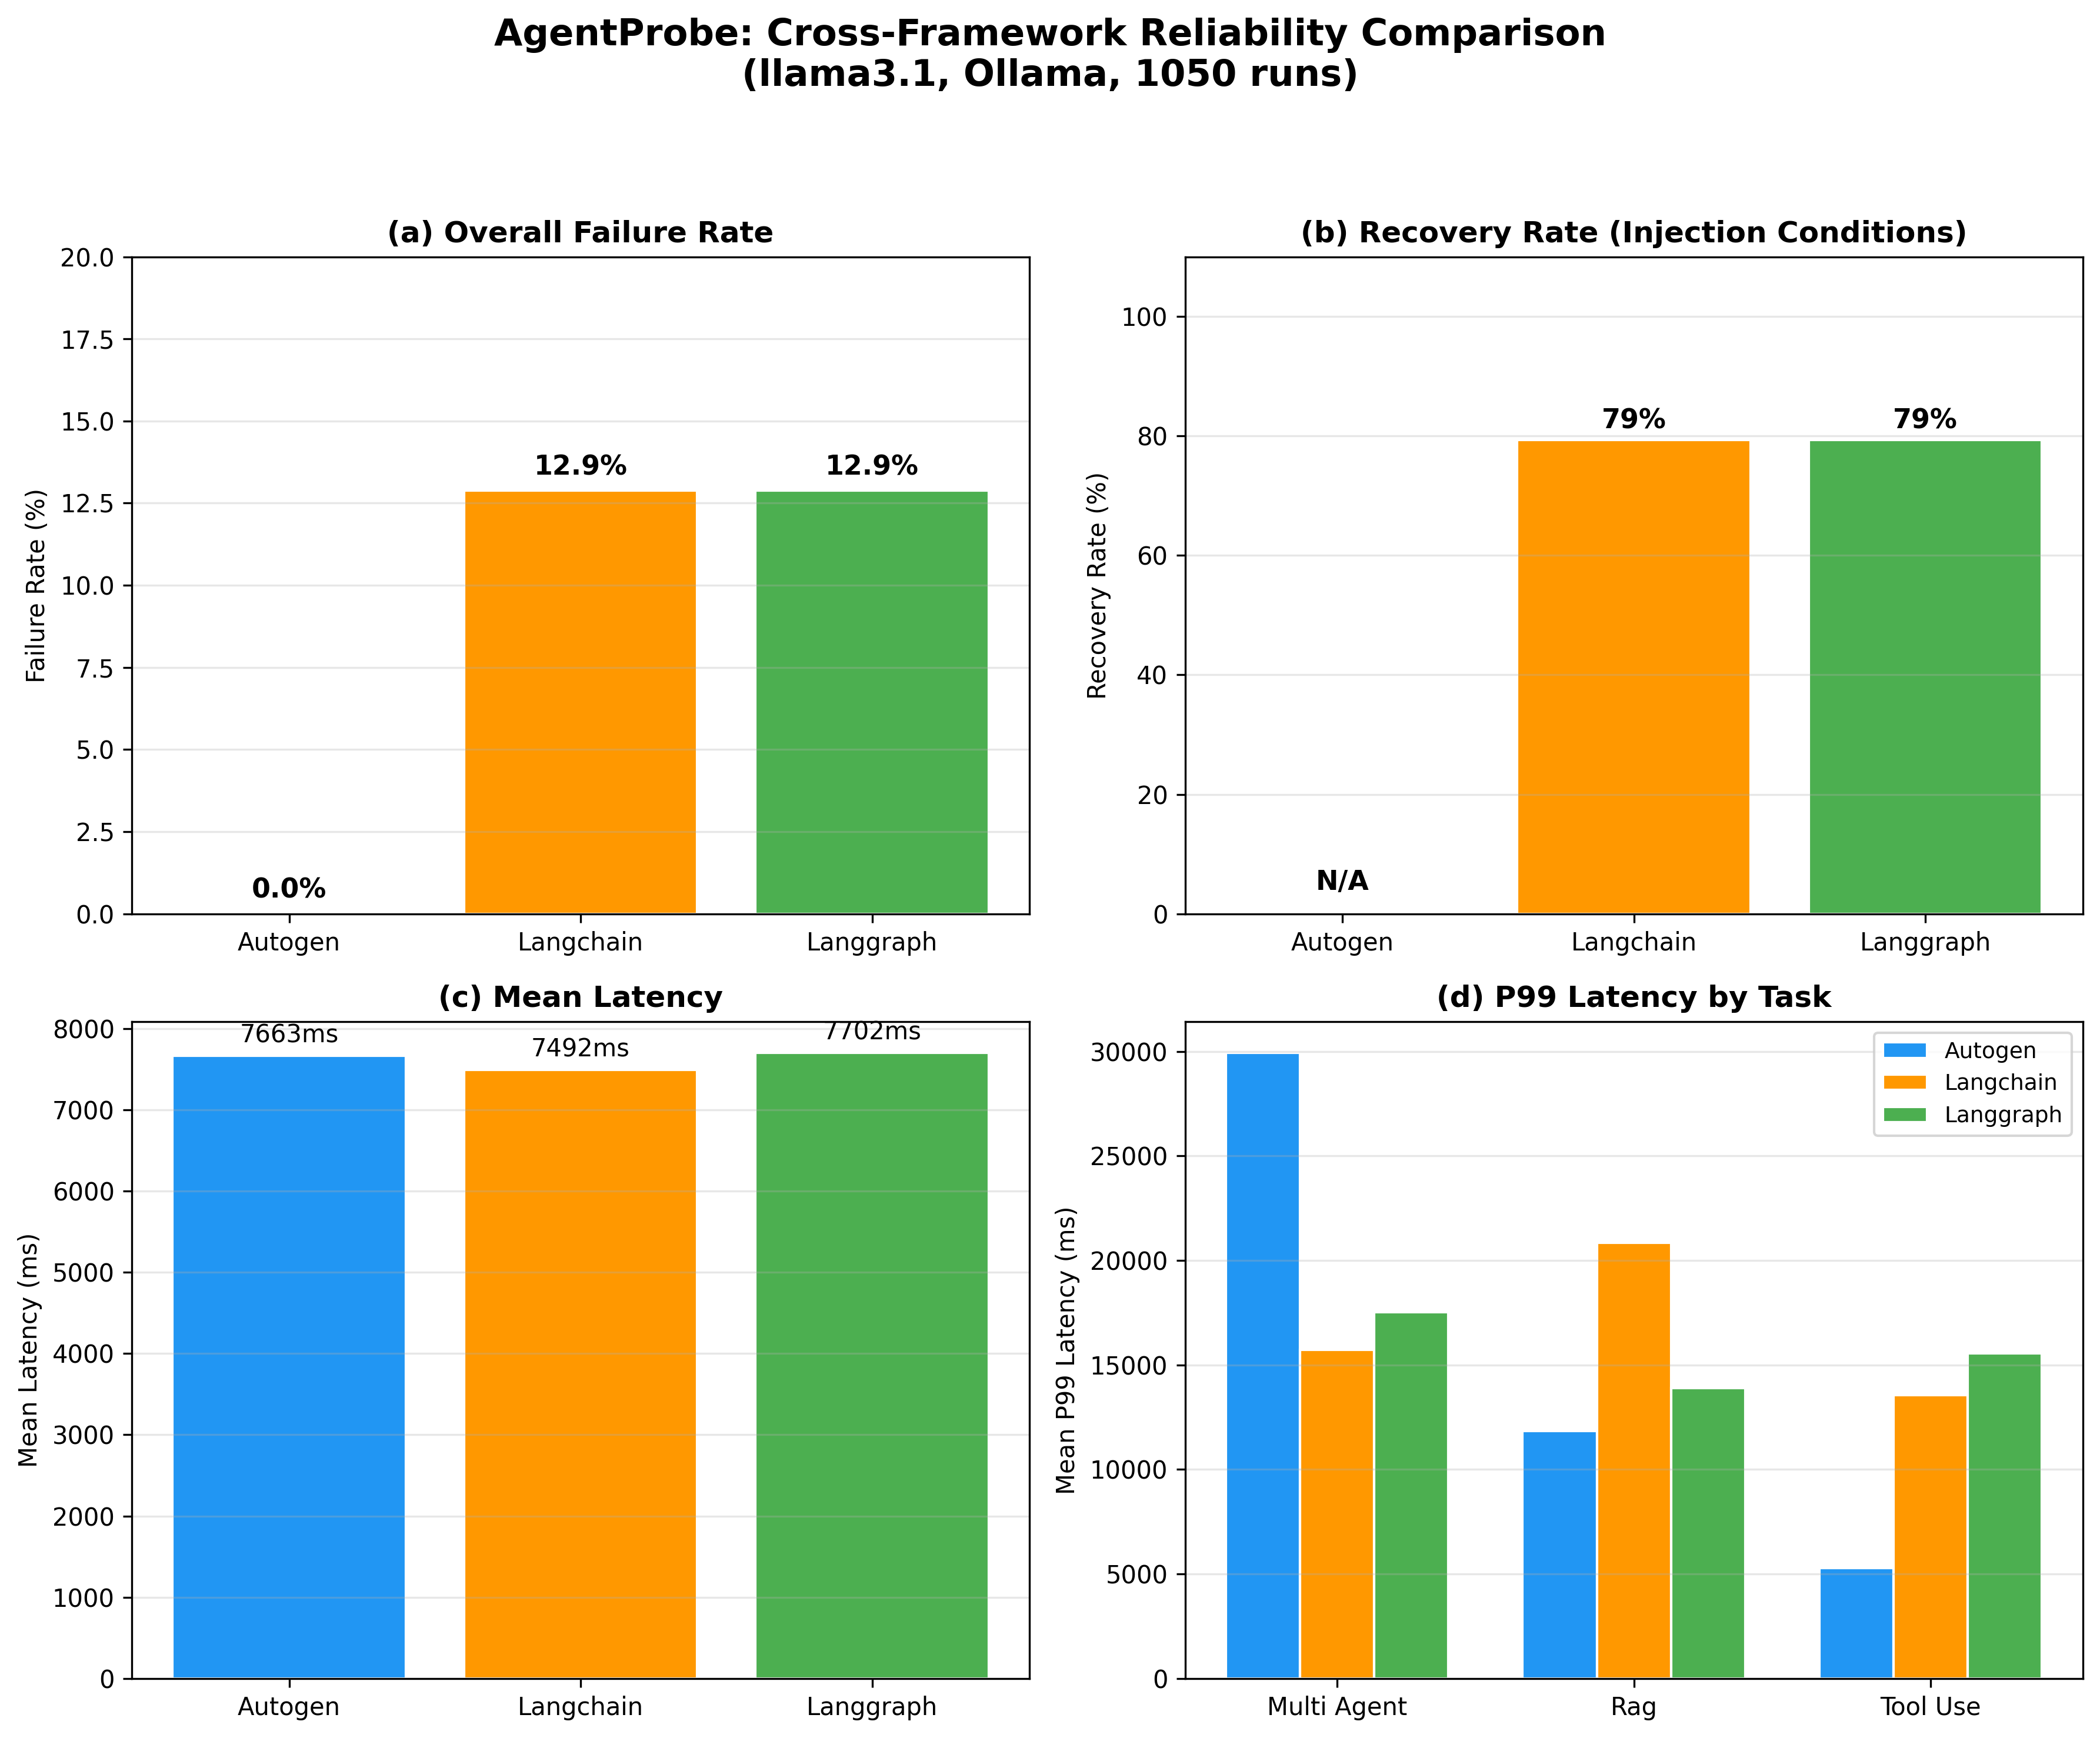
\includegraphics[width=\textwidth]{../experiments/plots/summary_dashboard.png}
  \caption{Summary dashboard showing cross-framework reliability comparison: (a)~overall failure rate, (b)~recovery rate under injection conditions, (c)~mean baseline latency (no injection), and (d)~P99 baseline latency by task type. Panels (c) and (d) use baseline-only data to avoid conflating real LLM inference latency with AutoGen's near-zero injection latency caused by tool bypass. Based on 1{,}050 runs across LangGraph, LangChain, and AutoGen with Llama~3.1 via Ollama.}\label{fig:dashboard}
\end{figure}

\subsection{Baseline Performance}

Under baseline conditions (no fault injection), all three frameworks achieve a 0\% failure rate [95\%~CI: 0.0--4.1\%] across all task types ($n = 90$ per framework for LangGraph/LangChain, $n = 30$ for AutoGen). Mean latency varies by task: tool use is fastest (LangGraph: 6.1\,s, LangChain: 6.0\,s), followed by RAG (8.0\,s, 11.4\,s) and multi-agent coordination (11.7\,s, 10.7\,s). AutoGen exhibits substantially higher and more variable latency, with mean latency ranging from 10.9\,s for tool use to 76.1\,s for multi-agent tasks, reflecting the overhead of its conversation-based protocol.

\subsection{Fault Tolerance Comparison}

\begin{figure}[htbp]
  \centering
  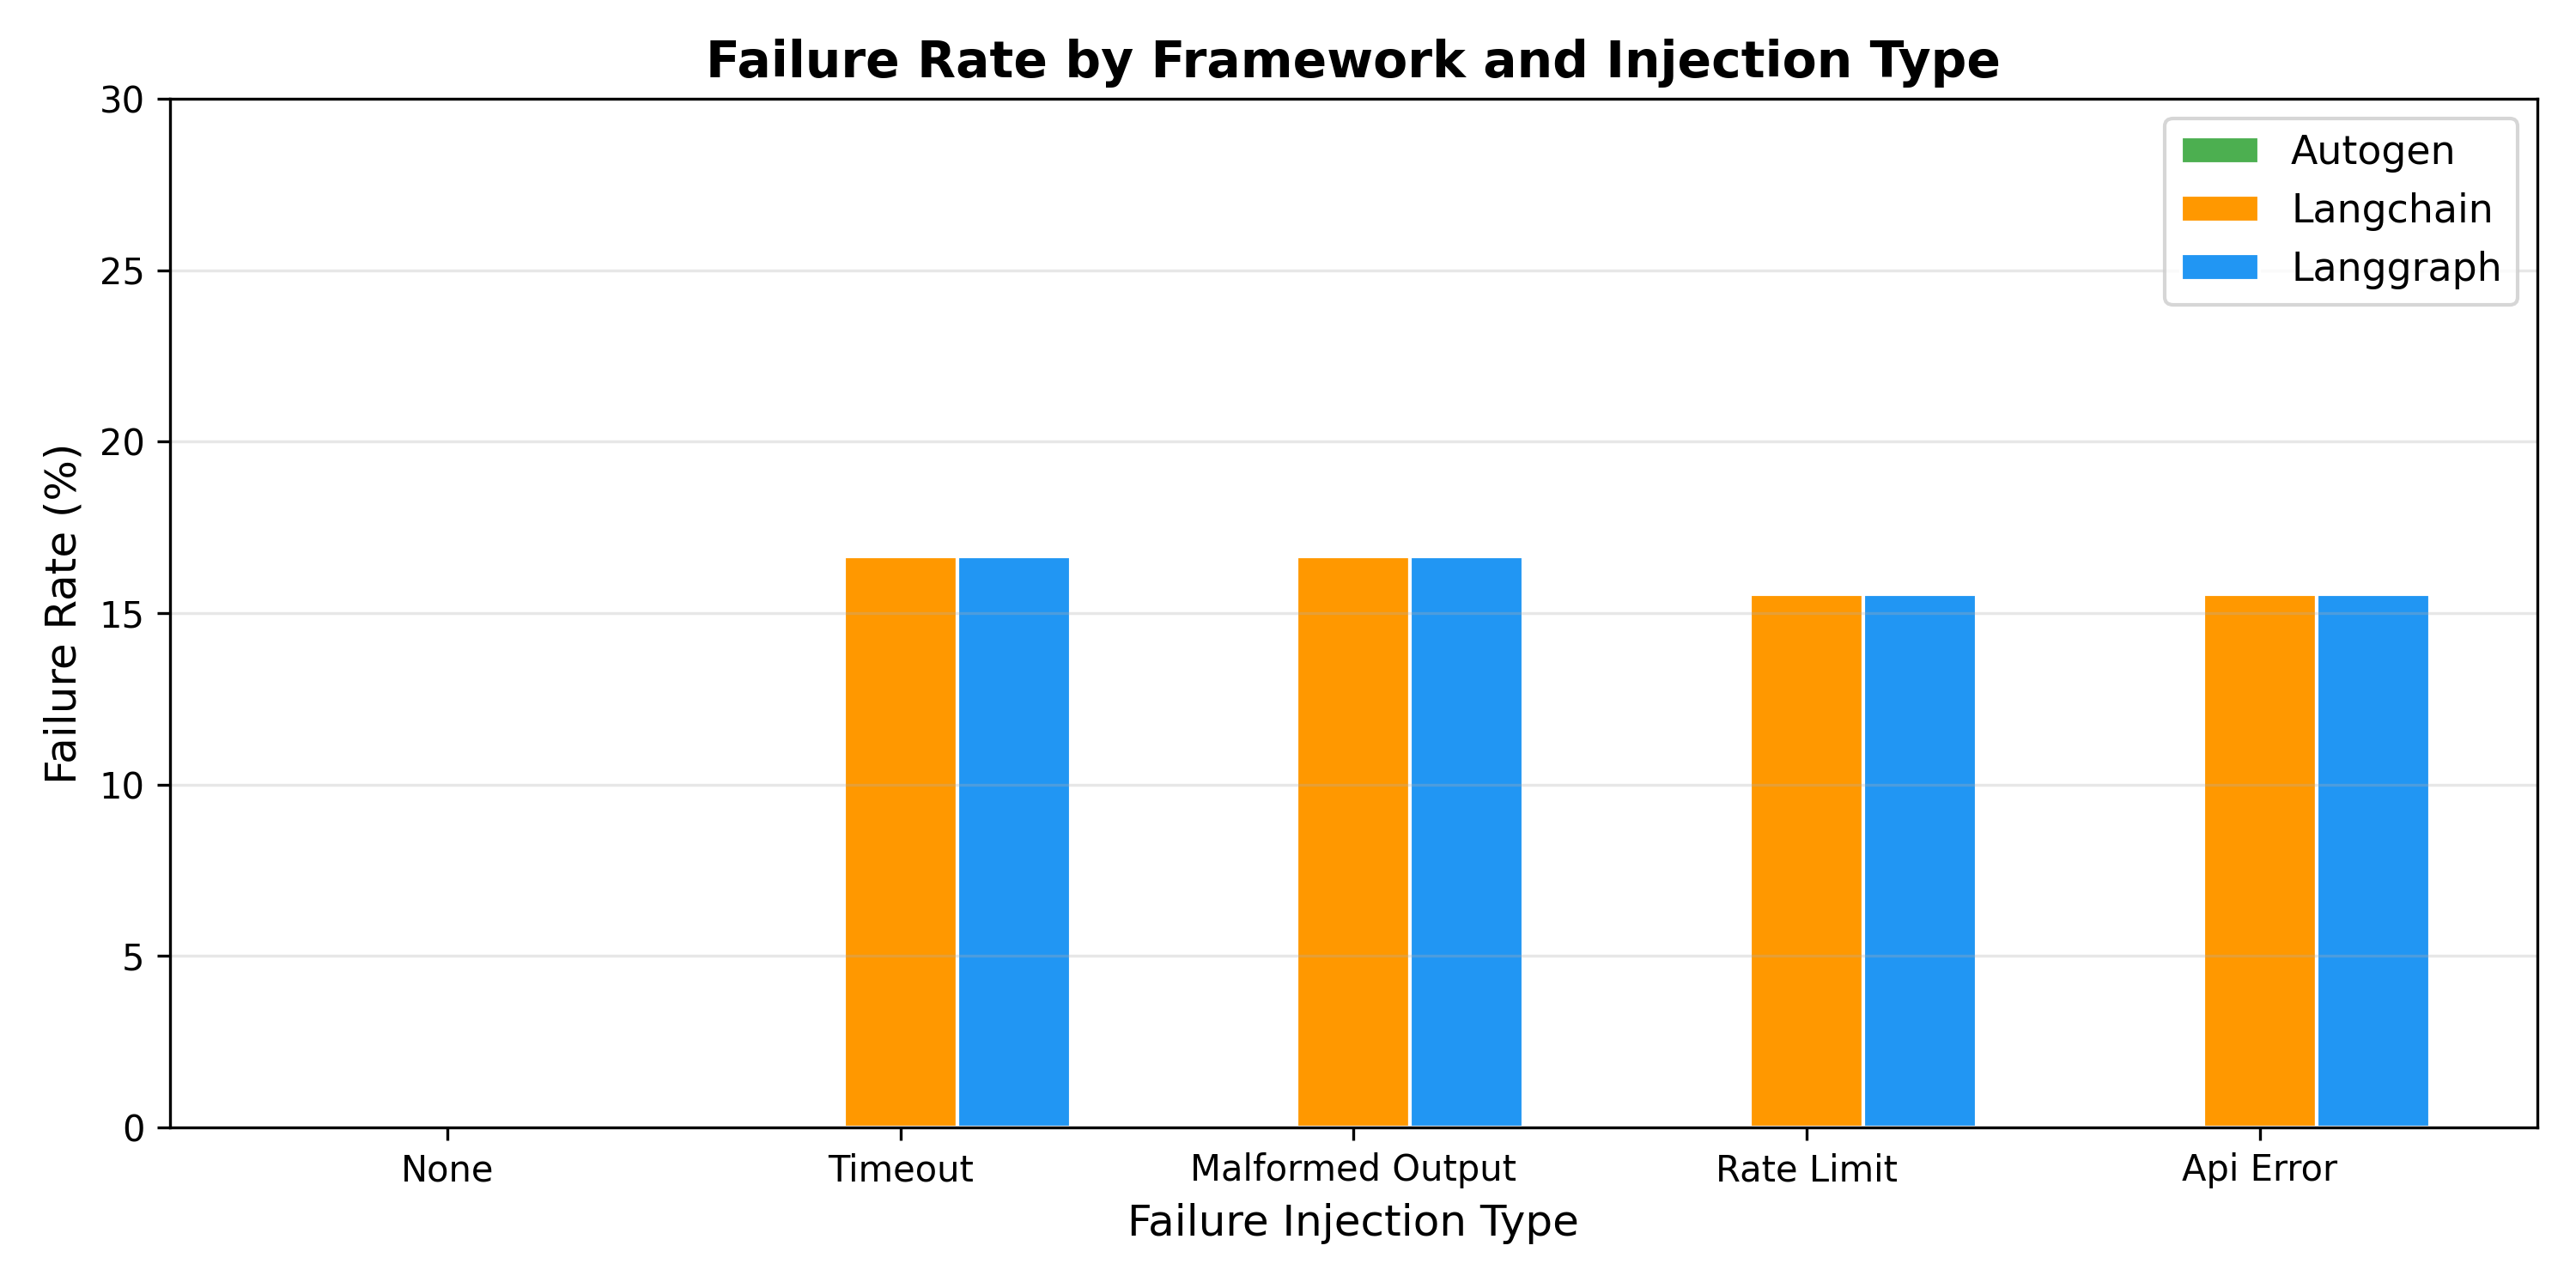
\includegraphics[width=\textwidth]{../experiments/plots/failure_rate_by_framework.png}
  \caption{Failure rate by framework and injection type. LangGraph and LangChain show matched failure rates under all injection conditions, while AutoGen reports 0\% across all conditions due to tool-execution bypass. Error bars omitted for clarity; 95\% Wilson score CIs are reported in the text.}\label{fig:sr_comparison}
\end{figure}

Under fault injection, LangGraph and LangChain both exhibit an overall failure rate of 12.9\% [95\%~CI: 10.1--16.3\%], with 58 failures out of 450 runs each. Timeout and malformed output injection produce failure rates of 16.7\% [10.4--25.7\%], while rate limit and API error injection yield 15.6\% [9.5--24.4\%]. The difference between LangGraph and LangChain is not statistically significant ($\chi^2$ test with Yates' correction, $p = 1.0$, Cohen's $h = 0.000$, negligible effect). This is expected: LangChain~v1.3+ internally delegates to LangGraph for agent execution, making them architecturally equivalent at the tool-calling layer.

AutoGen reports 0\% failure across all conditions [95\%~CI: 0.0--2.5\%, $n = 150$]. The difference versus LangGraph/LangChain is highly significant ($\chi^2$, $p < 0.0001$, Cohen's $h = 0.73$, medium effect).

\subsection{The Silent Failure Phenomenon}

Closer inspection of AutoGen traces reveals that the 0\% failure rate is an artifact: AutoGen with Llama~3.1 via Ollama does not produce function-call-formatted responses. The LLM responds directly to queries without invoking any tools, so the fault injectors are never triggered. This constitutes a \emph{silent failure}---the agent appears resilient but is not actually using its tools, producing answers from parametric knowledge alone.

This finding underscores a critical limitation of pass/fail metrics: an agent that bypasses its tools entirely will show perfect scores on fault-injection benchmarks while potentially producing less accurate or less grounded answers. AgentProbe's observability layer detects this through tool invocation counts in the trace data.

\subsection{Recovery Behavior}

\begin{figure}[htbp]
  \centering
  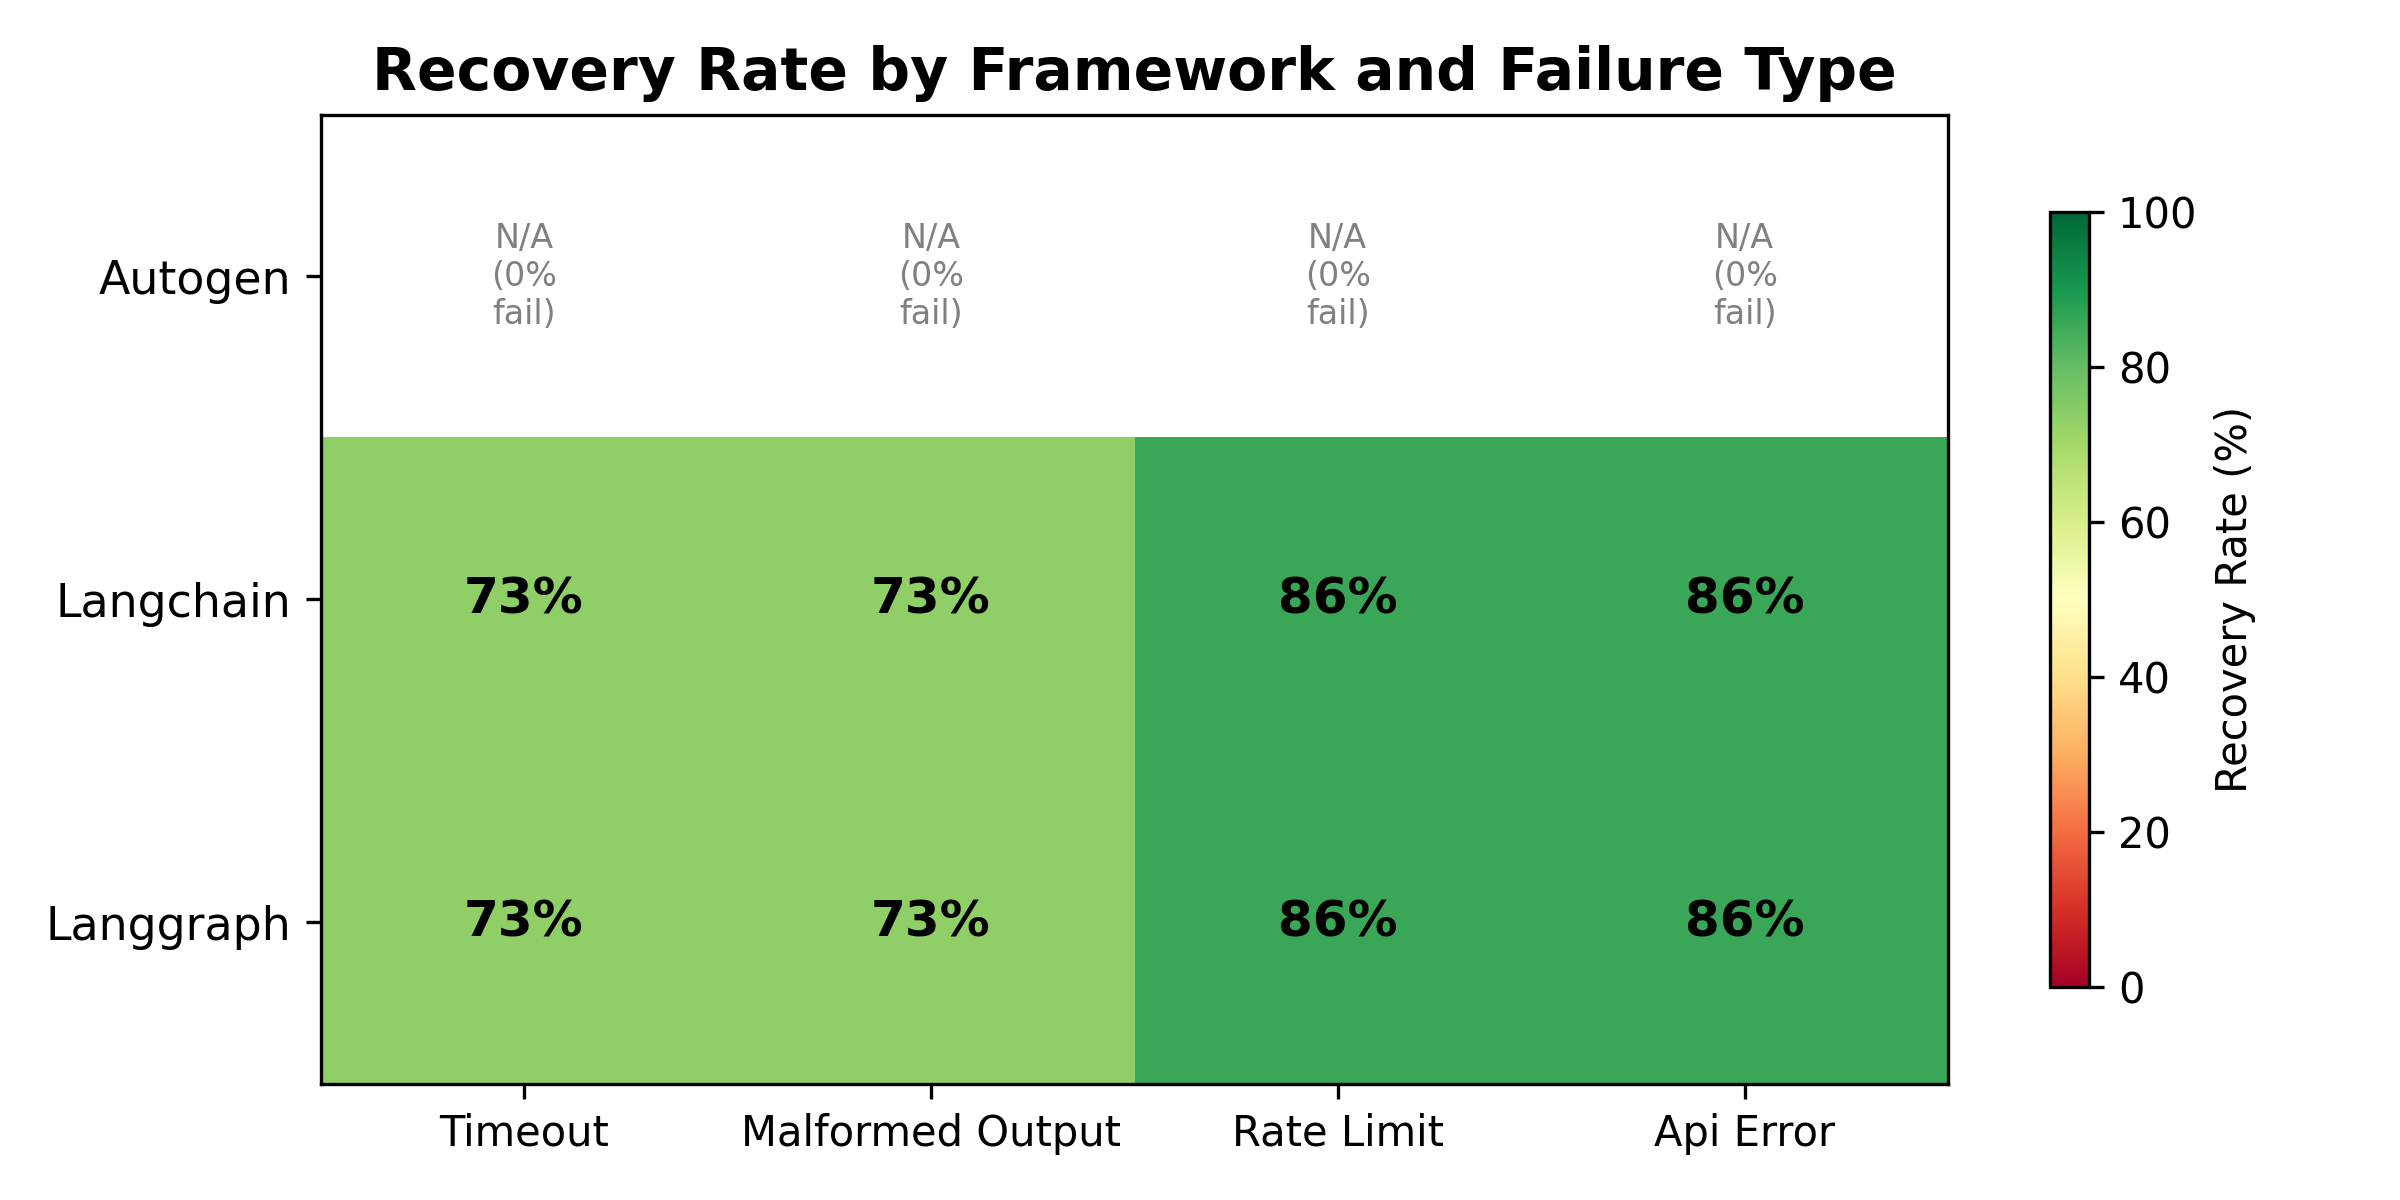
\includegraphics[width=\textwidth]{../experiments/plots/recovery_rate_heatmap.png}
  \caption{Recovery rate heatmap by framework and failure type. Rate limit and API error conditions show higher recovery (86\%) than timeout and malformed output (73\%). AutoGen shows N/A (no failures to recover from).}\label{fig:recovery}
\end{figure}

For LangGraph and LangChain, recovery rates differ by failure type. Rate limit and API error injections yield 86\% recovery, while timeout and malformed output injections yield 73\% recovery. This pattern is consistent across both frameworks and all task types: transient errors that produce clear error signals (HTTP~429, 503) are more recoverable than timeouts (which block execution) and malformed outputs (which may propagate silently through the reasoning chain).

\subsection{Latency Impact}

\begin{figure}[htbp]
  \centering
  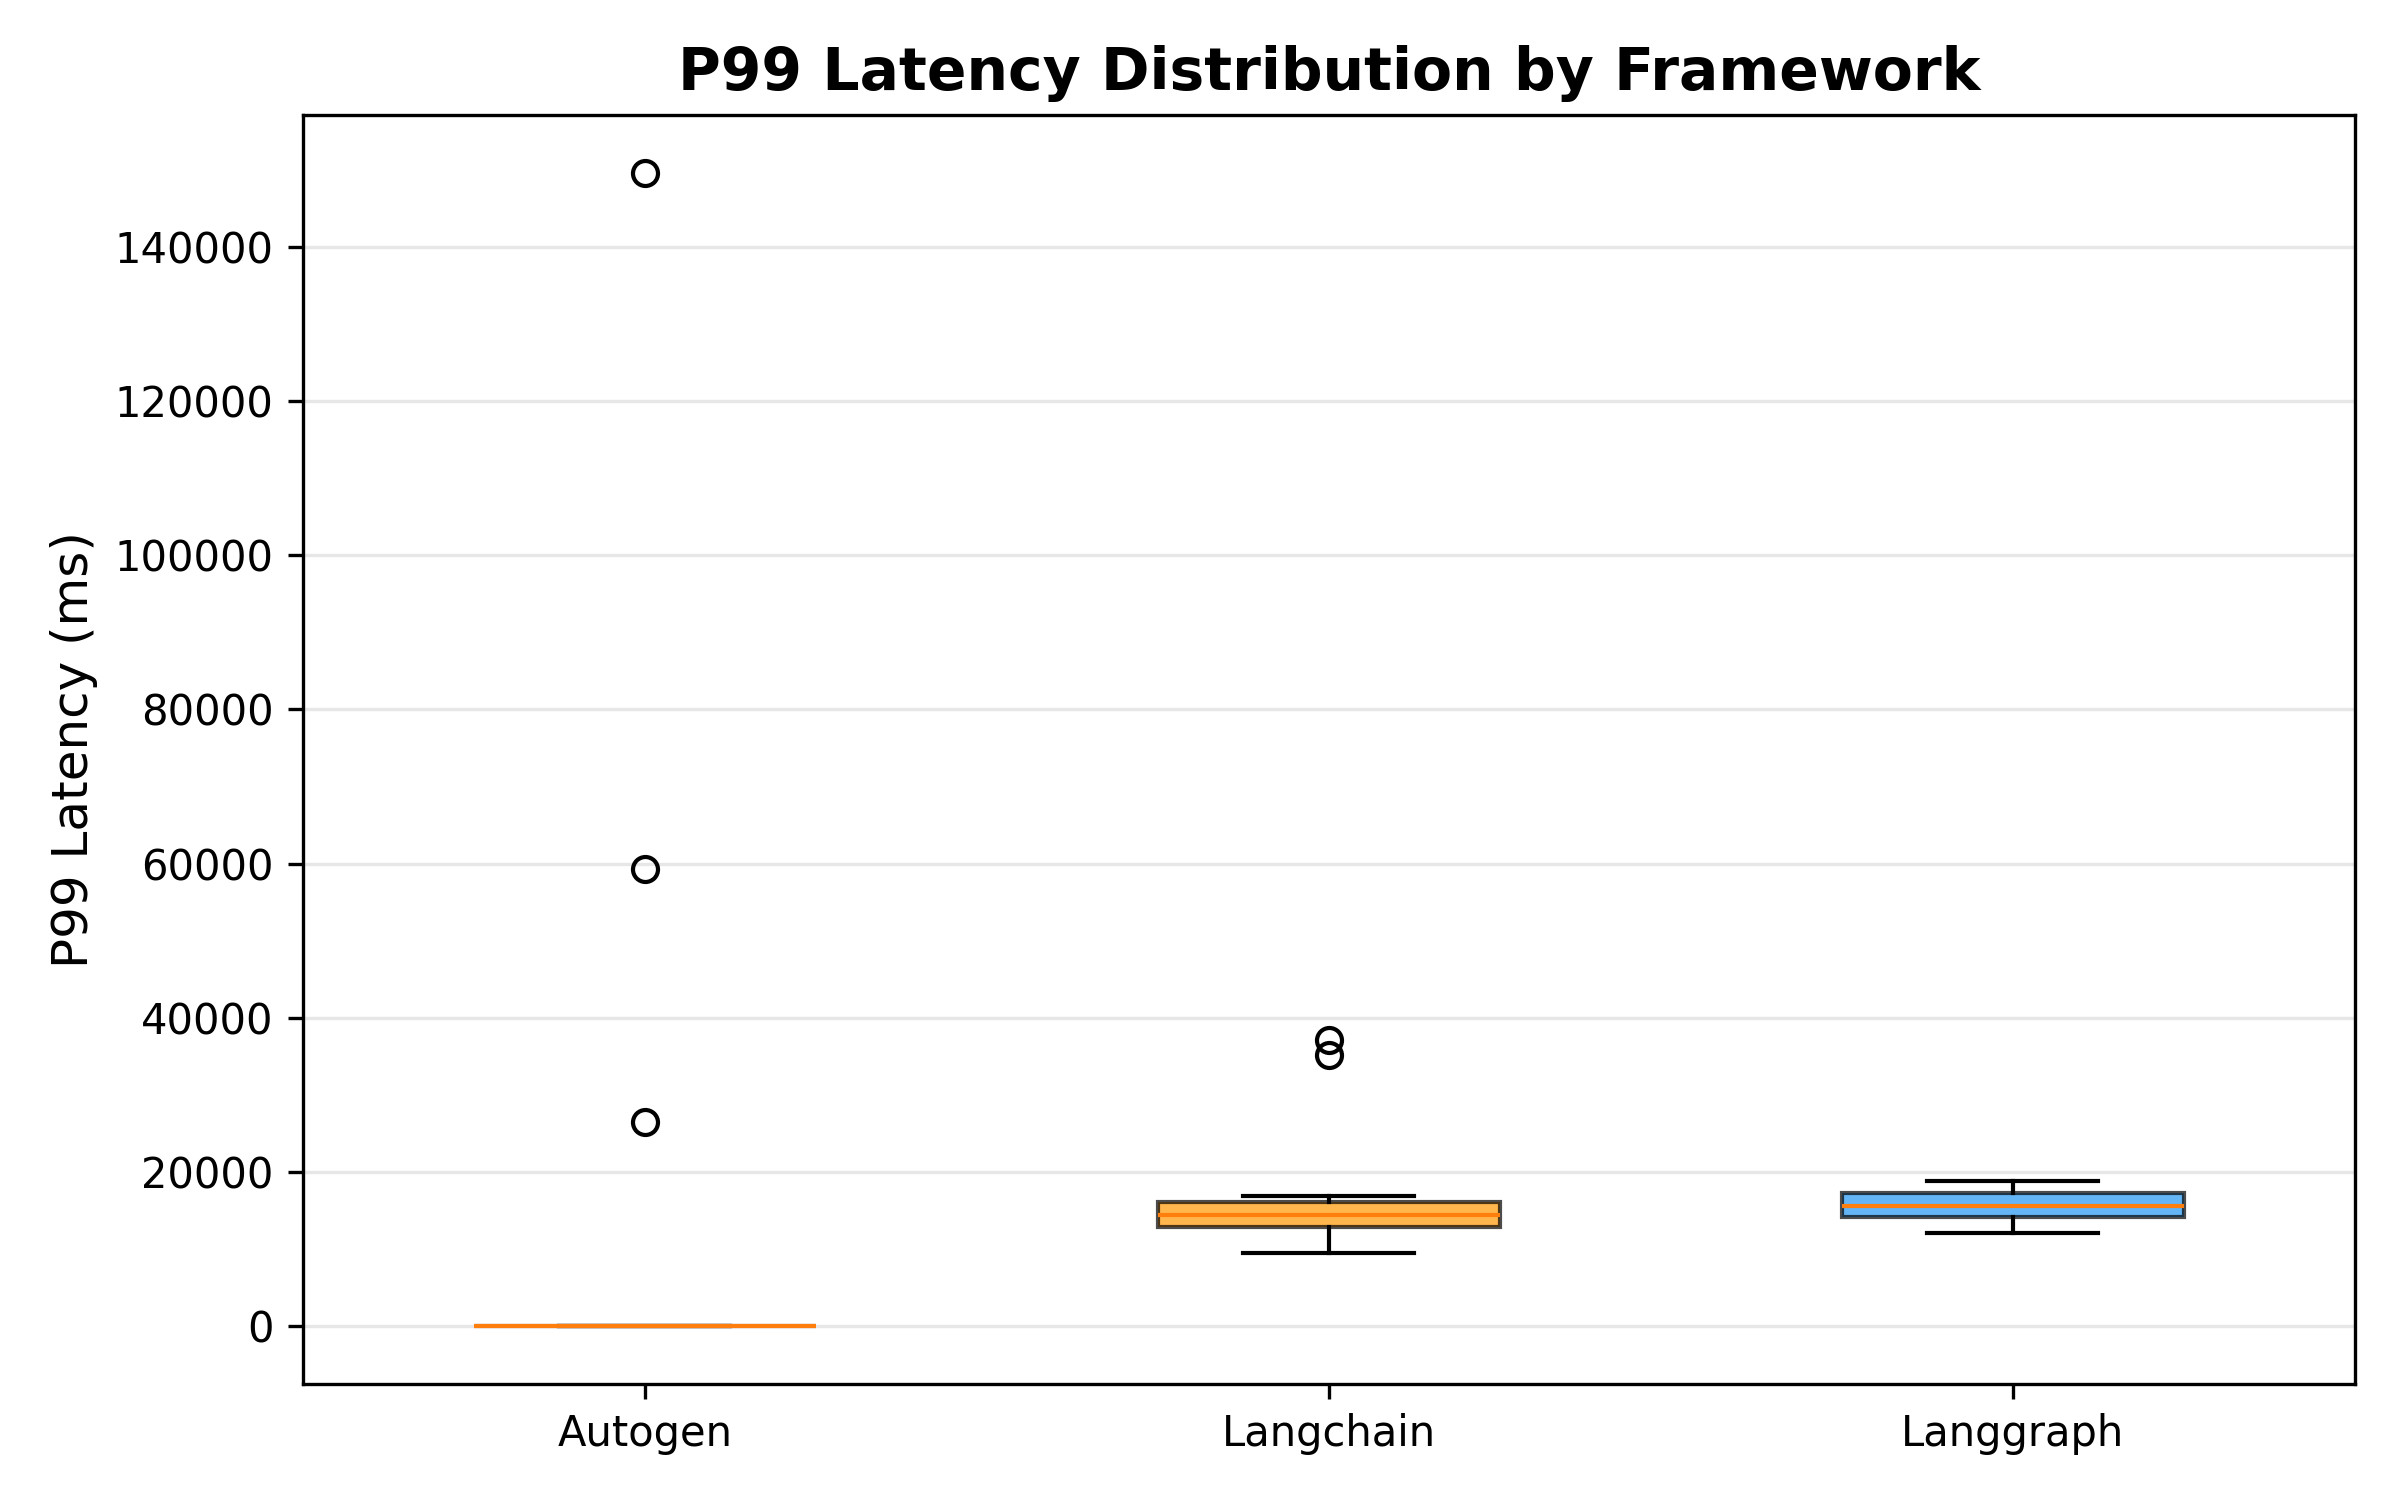
\includegraphics[width=0.8\textwidth]{../experiments/plots/latency_comparison.png}
  \caption{P99 latency distribution across frameworks. The omnibus Kruskal--Wallis test indicates a significant difference ($H = 11.65$, $p = 0.003$), driven by AutoGen's high variance in baseline conditions.}\label{fig:latency}
\end{figure}

Under baseline conditions (no injection), latency differs substantially across frameworks. LangGraph and LangChain exhibit similar mean latencies (8.6\,s and 9.4\,s respectively), while AutoGen is significantly slower (38.3\,s mean), with P99 reaching 149\,s for multi-agent tasks. The omnibus Kruskal--Wallis test confirms a significant difference in latency distributions ($H = 11.65$, $p = 0.003$). AutoGen's conversation-based protocol incurs substantial overhead for real LLM inference. Under injection conditions, AutoGen exhibits near-zero latency (6--27\,ms) because the agent bypasses tool execution entirely, producing fast but ungrounded responses---a further manifestation of the silent failure phenomenon.

\subsection{Summary of Statistical Comparisons}

\begin{table}[htbp]
\caption{Pairwise statistical comparisons between frameworks. Failure rate comparisons use the chi-squared test with Yates' correction; latency comparisons use the Mann--Whitney $U$ test.}\label{tab:pairwise}
\centering
\resizebox{\textwidth}{!}{%
\begin{tabular}{llcccc}
\toprule
\textbf{Comparison} & \textbf{Metric} & \textbf{Test} & \textbf{$p$-value} & \textbf{Effect Size} & \textbf{Magnitude} \\
\midrule
AutoGen vs LangChain   & Failure rate & $\chi^2$ (Yates) & $< 0.0001$ & $h = 0.73$ & Medium \\
AutoGen vs LangGraph   & Failure rate & $\chi^2$ (Yates) & $< 0.0001$ & $h = 0.73$ & Medium \\
LangChain vs LangGraph & Failure rate & $\chi^2$ (Yates) & $1.0$       & $h = 0.00$ & Negligible \\
\midrule
AutoGen vs LangChain   & Latency & Mann--Whitney $U$ & $0.004$ & $d = 0.01$ & Negligible \\
AutoGen vs LangGraph   & Latency & Mann--Whitney $U$ & $0.005$ & $d = 0.00$ & Negligible \\
LangChain vs LangGraph & Latency & Mann--Whitney $U$ & $0.245$ & $d = 0.09$ & Negligible \\
\bottomrule
\end{tabular}%
}
\end{table}


% ============================================================================
\section{Discussion}\label{sec:discussion}
% ============================================================================

\subsection{Architectural Implications}

Our results reveal three key architectural insights. First, the convergence of LangGraph and LangChain ($p = 1.0$) reflects a broader trend in the ecosystem: LangChain~v1.3+ delegates agent execution to LangGraph internally, making architectural differences at the tool-calling layer negligible. From a BDI perspective, both frameworks implement equivalent plan-selection and intention-reconsideration mechanisms for tool-augmented agents.

Second, AutoGen's tool-execution bypass exposes a critical gap in conversation-based architectures when paired with local models. The OpenAI-compatible API used by pyautogen does not enforce function-call formatting with Ollama-served models, causing the LLM to skip tool invocation entirely. This is analogous to a BDI agent that abandons its plans in favor of direct belief-based responses---functional but ungrounded.

Third, the differential recovery rates (86\% for rate limit/API error vs.\ 73\% for timeout/malformed output) suggest that agents handle failures with clear error signals better than failures that block execution or corrupt the reasoning chain. This motivates the design of agent middleware that converts ambiguous failures into explicit error messages.

\subsection{Toward Reliable Agent-Oriented Systems}

Based on our findings, we recommend: (1)~\textbf{tool invocation auditing} as a mandatory component of agent evaluation, to detect silent failure modes like tool-execution bypass; (2)~\textbf{explicit error wrapping} for tool calls, converting timeouts and malformed outputs into structured error responses that the LLM can reason about; (3)~\textbf{framework-agnostic fault injection} as part of CI/CD pipelines for agent systems; and (4)~\textbf{multi-metric evaluation} combining pass/fail rates with tool usage statistics, recovery rates, and latency distributions.

\subsection{Bridging Symbolic and Sub-Symbolic Agents}

The failure modes observed in LLM-based agents highlight capabilities that symbolic BDI agents handle naturally: explicit goal management prevents infinite loops, formal plan libraries enable structured recovery, and logical state representations resist corruption. Conversely, LLM-based agents excel at flexible tool use and natural language understanding, where symbolic agents struggle.

Our taxonomy suggests a natural division of labor: BDI-style goal management and plan selection could address orchestration errors (infinite loops, wrong branching) and context degradation (by maintaining explicit state), while LLM-based reasoning handles flexible tool use and natural language understanding. The silent failure phenomenon observed in AutoGen further motivates hybrid designs: a BDI layer could enforce tool invocation requirements as part of its plan structure, preventing the LLM from bypassing tools. AgentProbe's fault injectors provide a testbed for evaluating such hybrid architectures.

\subsection{Limitations}

\begin{itemize}
  \item Our study evaluates three frameworks; results may not generalize to all agent architectures (e.g., CrewAI, DSPy).
  \item Fault injection probabilities are uniform ($p = 0.15$--$0.20$); production failure patterns may be bursty or correlated.
  \item We use a single LLM backend (Llama~3.1 8B); larger models or commercial APIs (GPT-4, Claude) may exhibit different resilience characteristics, particularly for tool-calling format compliance.
  \item The convergence of LangChain and LangGraph is version-specific (LangChain~v1.3+); earlier versions with the deprecated \texttt{AgentExecutor} may show different behavior.
  \item AutoGen's tool-execution bypass is specific to the pyautogen~0.1.14 + Ollama combination; the newer AutoGen~0.4 (AG2) SDK may handle local models differently.
\end{itemize}

\subsection{Threats to Validity}

\paragraph{Internal Validity.} The use of controlled fault injection with fixed probabilities and a fixed seed (42) ensures reproducibility but may not capture the complexity of real-world failure patterns. We mitigate this by using 10--30 runs per condition and reporting Wilson score confidence intervals.

\paragraph{External Validity.} Our benchmark tasks are designed to be representative but cannot cover all possible agent applications. We select tasks that exercise the core capabilities (tool use, RAG, multi-agent coordination) common to most production deployments.

\paragraph{Construct Validity.} Our metrics (success rate, recovery rate, etc.) are standard in reliability engineering but may not capture all dimensions of agent quality. We supplement quantitative metrics with qualitative trace analysis.


% ============================================================================
\section{Conclusions and Future Work}\label{sec:conclusion}
% ============================================================================

This paper presented \agentprobe{}, an open-source toolkit for systematically evaluating the reliability of LLM-based intelligent agents through controlled fault injection and observability. We introduced a five-category failure taxonomy covering tool call faults, orchestration errors, context degradation, latency anomalies, and output consistency violations. Through a comparative empirical study of LangGraph, LangChain, and AutoGen across 1{,}050 experiment runs, we demonstrated that: (1)~conventional pass/fail metrics can mask critical architectural weaknesses such as tool-execution bypass; (2)~LangGraph and LangChain exhibit equivalent fault tolerance at the tool-calling layer, reflecting their shared internal architecture; (3)~recovery rates vary systematically by failure type, with transient errors recovering better than blocking or corrupting failures; and (4)~systematic fault injection with multi-metric evaluation is essential for trustworthy agent assessment.

Our contributions advance the understanding of how sub-symbolic intelligent agents fail and recover, providing empirical grounding for the design of more robust agent-oriented systems. The open-source release of \agentprobe{} enables the research community to reproduce our results and extend the evaluation to additional frameworks, failure modes, and application domains.

\paragraph{Future Work.}
Several directions merit further investigation:
\begin{itemize}
  \item \textbf{Hybrid architectures:} Integrating BDI-style formal reasoning with LLM-based agents to address the failure modes identified in our taxonomy.
  \item \textbf{Adaptive fault injection:} Developing intelligent fault injection strategies that target framework-specific weak points identified through initial profiling.
  \item \textbf{Multi-model evaluation:} Extending the study to compare resilience across different LLM backends (e.g., GPT-4, Claude, Llama, Mistral).
  \item \textbf{Production telemetry integration:} Connecting \agentprobe{}'s observability layer with production monitoring systems for continuous reliability assessment.
  \item \textbf{Automated recovery synthesis:} Using the failure taxonomy to automatically generate recovery strategies for detected failure patterns.
\end{itemize}

\vspace{6pt}

% ============================================================================
% Supplementary Materials, Author Contributions, Funding, etc.
% ============================================================================

\authorcontributions{Conceptualization, methodology, software, investigation, writing---original draft preparation, C.J.; supervision, writing---review and editing, S.P. and E.P. All authors have read and agreed to the published version of the manuscript.}

\funding{This research received no external funding.}

\dataavailability{The \agentprobe{} toolkit, benchmark tasks, and experimental scripts are available as open-source software at \url{https://github.com/chhayankjain/AgentProbe}.}

\conflictsofinterest{The authors declare no conflicts of interest.}

% ============================================================================
% References
% ============================================================================

\reftitle{References}

\begin{thebibliography}{99}

\bibitem{wooldridge2009introduction}
Wooldridge, M.
\newblock \textit{An Introduction to MultiAgent Systems}, 2nd~ed.;
\newblock John Wiley \& Sons: Chichester, UK, 2009.

\bibitem{wooldridge1995intelligent}
Wooldridge, M.; Jennings, N.R.
\newblock Intelligent agents: theory and practice.
\newblock \textit{The Knowledge Engineering Review} \textbf{1995}, \textit{10}, 115--152.

\bibitem{rao1995bdi}
Rao, A.S.; Georgeff, M.P.
\newblock BDI agents: From theory to practice.
\newblock In Proceedings of the First International Conference on Multi-Agent Systems (ICMAS-95), San Francisco, CA, USA, 12--14 June 1995; pp.~312--319.

\bibitem{yao2023react}
Yao, S.; Zhao, J.; Yu, D.; Du, N.; Shafran, I.; Narasimhan, K.; Cao, Y.
\newblock ReAct: Synergizing reasoning and acting in language models.
\newblock In Proceedings of the International Conference on Learning Representations (ICLR), Kigali, Rwanda, 1--5 May 2023.

\bibitem{wei2022chain}
Wei, J.; Wang, X.; Schuurmans, D.; Bosma, M.; Ichter, B.; Xia, F.; Chi, E.; Le, Q.; Zhou, D.
\newblock Chain-of-thought prompting elicits reasoning in large language models.
\newblock In \textit{Advances in Neural Information Processing Systems} (NeurIPS); 2022; Vol.~35, pp.~24824--24837.

\bibitem{langgraph2024}
LangChain, Inc.
\newblock LangGraph: Build Stateful, Multi-Actor Applications with LLMs, 2024.

\bibitem{langchain2023}
Chase, H.
\newblock LangChain: Building applications with LLMs through composability, 2023.

\bibitem{wu2023autogen}
Wu, Q.; Bansal, G.; Zhang, J.; Wu, Y.; Li, B.; Zhu, E.; Jiang, L.; Zhang, X.; Zhang, S.; Liu, J.; et~al.
\newblock AutoGen: Enabling next-gen LLM applications via multi-agent conversation.
\newblock \textit{arXiv preprint arXiv:2308.08155} \textbf{2023}.

\bibitem{opentelemetry2024}
OpenTelemetry Authors.
\newblock OpenTelemetry---An observability framework for cloud-native software, 2024.

\bibitem{bordini2007programming}
Bordini, R.H.; H{\"u}bner, J.F.; Wooldridge, M.
\newblock \textit{Programming Multi-Agent Systems in AgentSpeak using Jason};
\newblock John Wiley \& Sons: Chichester, UK, 2007.

\bibitem{winikoff2005jack}
Winikoff, M.
\newblock JACK intelligent agents: An industrial strength platform.
\newblock In \textit{Multi-Agent Programming}; Springer: Boston, MA, USA, 2005; pp.~175--193.

\bibitem{stoyanov2024agents}
Stoyanov, S.; Doycheva, A.; Tabakova-Komsalova, V.
\newblock Intelligent agents and their applications in modern computing.
\newblock \textit{Future Internet} \textbf{2024}, \textit{16}.

\bibitem{hsueh1997fault}
Hsueh, M.-C.; Tsai, T.K.; Iyer, R.K.
\newblock Fault injection techniques and tools.
\newblock \textit{Computer} \textbf{1997}, \textit{30}, 75--82.

\bibitem{basiri2016chaos}
Basiri, A.; Behnam, N.; de~Rooij, R.; Hochstein, L.; Kosewski, L.; Reynolds, J.; Rosenthal, C.
\newblock Chaos engineering.
\newblock \textit{IEEE Software} \textbf{2016}, \textit{33}, 35--41.

\bibitem{chaostoolkit2024}
ChaosIQ.
\newblock Chaos Toolkit---An Open API for Chaos Engineering, 2024.

\bibitem{goodfellow2015explaining}
Goodfellow, I.J.; Shlens, J.; Szegedy, C.
\newblock Explaining and harnessing adversarial examples.
\newblock In Proceedings of the International Conference on Learning Representations (ICLR), San Diego, CA, USA, 7--9 May 2015.

\bibitem{ribeiro2020beyond}
Ribeiro, M.T.; Wu, T.; Guestrin, C.; Singh, S.
\newblock Beyond accuracy: Behavioral testing of NLP models with CheckList.
\newblock In Proceedings of the 58th Annual Meeting of the Association for Computational Linguistics (ACL), Online, 5--10 July 2020; pp.~4902--4912.

\bibitem{hendrycks2021measuring}
Hendrycks, D.; Burns, C.; Basart, S.; Zou, A.; Mazeika, M.; Song, D.; Steinhardt, J.
\newblock Measuring massive multitask language understanding.
\newblock In Proceedings of the International Conference on Learning Representations (ICLR), Virtual Event, 3--7 May 2021.

\bibitem{chen2021evaluating}
Chen, M.; Tworek, J.; Jun, H.; Yuan, Q.; Pinto, H.P.d.O.; Kaplan, J.; Edwards, H.; Burda, Y.; Joseph, N.; Brockman, G.; et~al.
\newblock Evaluating large language models trained on code.
\newblock \textit{arXiv preprint arXiv:2107.03374} \textbf{2021}.

\bibitem{liu2023agentbench}
Liu, X.; Yu, H.; Zhang, H.; Xu, Y.; Lei, X.; Lai, H.; Gu, Y.; Ding, H.; Men, K.; Yang, K.; et~al.
\newblock AgentBench: Evaluating LLMs as agents.
\newblock In Proceedings of the International Conference on Learning Representations (ICLR), Vienna, Austria, 7--11 May 2024.

\bibitem{yao2024tau}
Yao, S.; et~al.
\newblock $\tau$-bench: A benchmark for tool-agent-user interaction in real-world domains.
\newblock \textit{arXiv preprint} \textbf{2024}.

\bibitem{zhou2024webarena}
Zhou, S.; Xu, F.F.; Zhu, H.; Zhou, X.; Lo, R.; Sridhar, A.; Cheng, X.; Bisk, Y.; Fried, D.; Alon, U.; et~al.
\newblock WebArena: A realistic web environment for building autonomous agents.
\newblock In Proceedings of the International Conference on Learning Representations (ICLR), Vienna, Austria, 7--11 May 2024.

\bibitem{openllmetry2024}
Traceloop.
\newblock OpenLLMetry---Open-source observability for LLM applications, 2024.

\end{thebibliography}

\end{document}
